% !TEX root = ../main.tex
\section{Experiment}
\label{section:experiment}
In the following, we explain the framework we use to evaluate the approaches introduced above. After describing the experiment on which our models are trained, we illustrate different network architectures and hyperparameters. This is followed by a specification of the methods we apply to incorporate physical constraints into the learning process. 
\begin{figure}[H]
	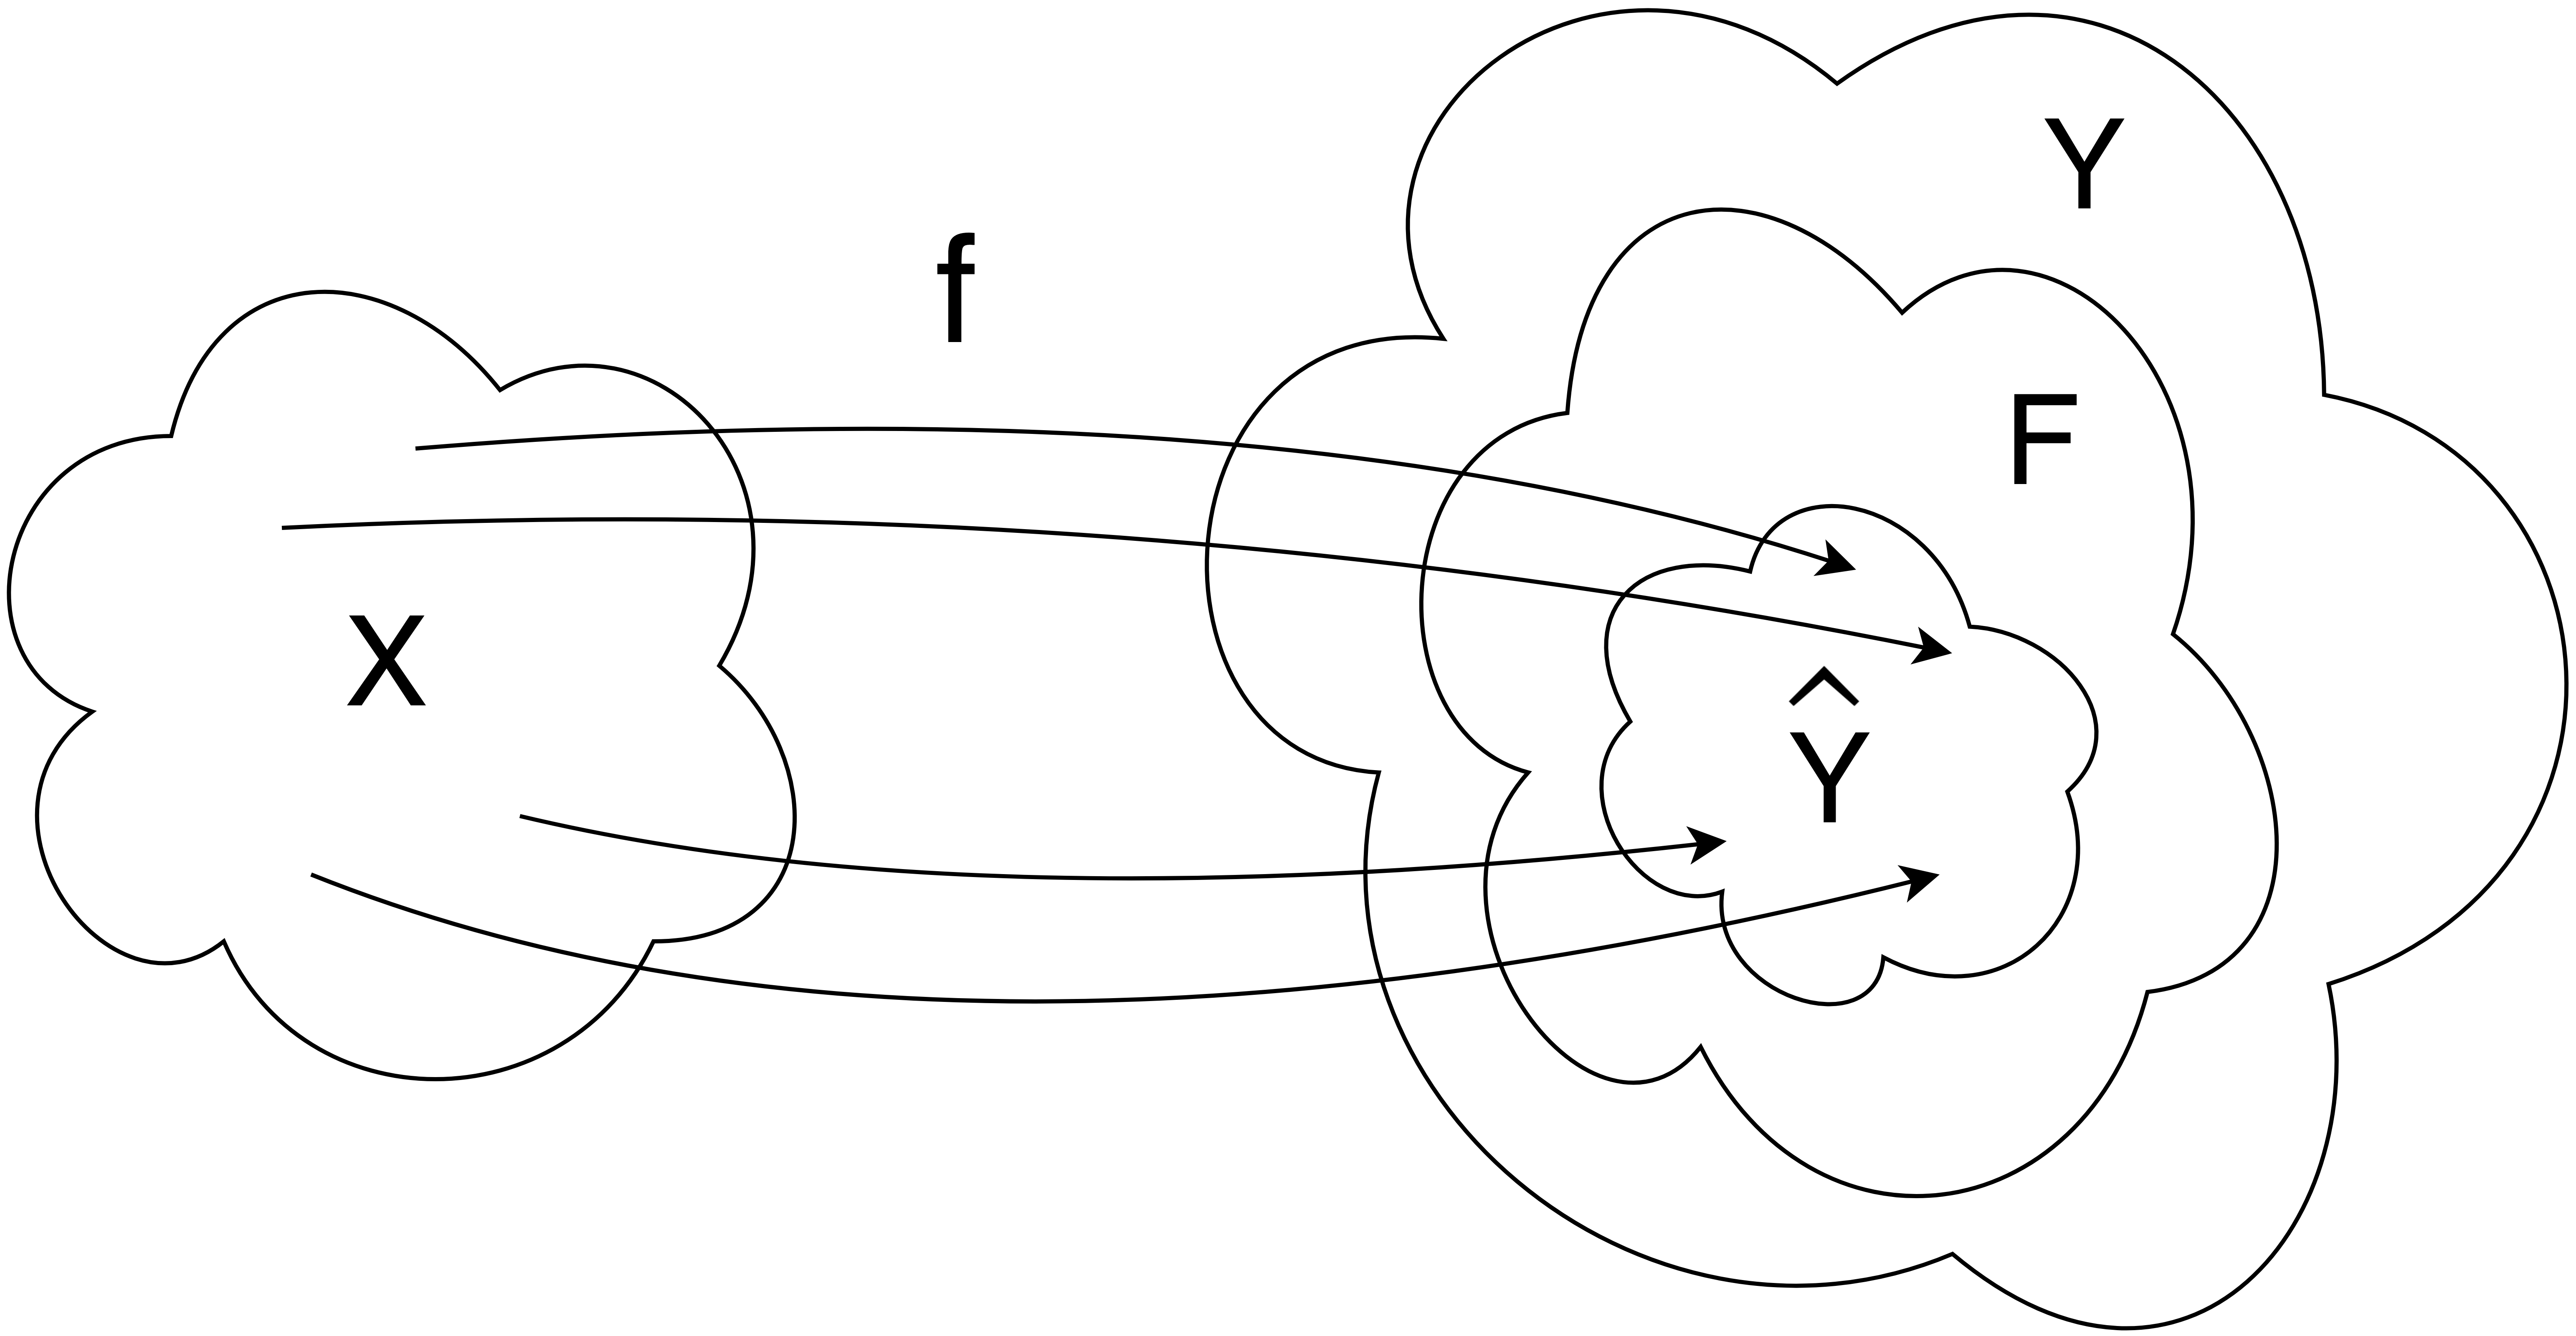
\includegraphics[width=\linewidth]{f_map}
	\caption{Visualisation of a function $f$ mapping from $X$ to $\hat{Y}$. $F$ denotes the physically feasible set and $Y$ a larger space for which we know that $\hat{Y} \subseteq Y$.}
	\label{fig:f_map}
\end{figure}
Before choosing an experiment to test our approaches on, we need to look at the structure of a learning problem. 
In general, a learning problem is the task of creating a function $\hat{f}_\theta: X \to Y$ with a model parameterised by $\theta$ that approximates the ground truth function $f: X \to \hat{Y}$, which maps given inputs of the domain $X$ to the corresponding output in the codomain $\hat{Y}$. An example for a ground truth function is visualised in Figure \ref{fig:f_map}. Usually, we do not have access to the ground truth $f$, but instead try to learn it with the help of a set of data points $D \subseteq \{(x, y), x \in X, y \in \hat{Y} | f(x) = y\}$. Since we know that any ground truth satisfies all physical constraints, the set of outputs $\hat{Y}$ of $f$ is a subset of the set of all feasible points $F$, meaning that $\hat{Y} \subseteq F$. However, when trying to learn the function $\hat{f}_\theta: X \to \hat{Y}$, we usually do not know the set of outputs $\hat{Y}$. Therefore, we start with the representation $\hat{f}_\theta: X \to Y$, where $Y$ is a much larger space for which we know that $\hat{Y} \subseteq F \subseteq Y$. To give an example, we look at the following function:

\begin{equation}
\label{example_fn}
\begin{aligned}
g: &[0, \pi] \to [0, 1]\\
&x \mapsto \sin(x)
\end{aligned}
\end{equation}
Even though the function $g$ only maps values of the domain space $X = [0, \pi]$ to $\hat{Y} = [0, 1]$, feasible solutions contain all values between $-1$ and $1$, namely $F = [-1, 1]$, since we know that the function $\sin$ only outputs values in this range. Note that for this example, one could start with a model function $\hat{f}_\theta: X \to \hat{Y}$ parameterised by $\theta$ mapping only to $\hat{Y} = [0, 1]$, for example by applying the sigmoid function $\sigma(x) = 1 / (1 + e^{-x})$ to any predicted output. However, the set of ground truth outputs of real world problems is usually very complicated, which makes it impossible to initialise the model function $\hat{f}_\theta$ to only output values in $\hat{Y}$. For this reason, when trying to train a model $\hat{f}_\theta$ without any prior knowledge about the ground truth function $f$, we start by constructing a function $\hat{f}_\theta: X \to Y$ that maps inputs to the larger space $Y$. In our example of the function $g$, one would initially construct a model function $\hat{f}_\theta: [0, \pi] \to \mathbb{R}$ mapping inputs to the real numbers.\\
\indent By incorporating physical constraints into the training process of deep learning models, we try to reduce the distance between the predictions $y_{pred} \in Y$ and the correct values $\hat{y}_{true} \in \hat{Y}$ by training the model to output values in or close to the feasible region $F$.\\
\indent Since it can be difficult to break down the effects of incorporating knowledge about physical constraints on a deep learning model, the previously introduced methods have to be applied to a simple, yet not trivial problem. For measuring how well predictions align with the given physical constraints, we introduce the term \textit{realistic} to describe predictions with no or small constraint violations. By analysing the behaviour of our model, we aim to show that incorporating physical constraints contributes in the following ways:
\begin{itemize}
	\item Improve model performance,
	\item Create more realistic predictions,
	\item Decrease required amount of learning data.
\end{itemize}
A well fitting problem that satisfies both simplicity and the existence of physical constraints is provided by the task of learning a rotation. A rotation is a function that takes coordinates of a point together with rotation angles as input and outputs the coordinates of the rotated point.  The function can be described as a multiplication of a rotation matrix, which only depends on the rotation angle, and the point to be rotated. Rotations are invariant with respect to the L2-norm, meaning that the norm of the rotated point equals the norm of the input point. In addition, the determinant of the rotation matrix equals one. These two properties serve as physical constraints. Since the rotation problem satisfies the required characteristics, we use it to evaluate the previously introduced methods for incorporating physical constraints. The rotation problem itself is explained in more detail in the following section.

\subsection{Problem formulation}
In order to show the desired improvements, we apply the introduced methods to the rotation problem in both two and three dimensions. Formally, a rotation function maps a point $\vec{x}$ and rotation angles $\vec{\alpha}$ to a target point $\vec{y}$:
\begin{equation}
\label{rot_fn}
\begin{aligned}
rot: \,\,&\mathbb{R}^{d} \times [- \pi, \pi] ^{d-1} \to \mathbb{R}^{d}\\
&(\vec{x}, \vec{\alpha}) \mapsto rot(\vec{x}, \vec{\alpha}) = \vec{y},
\end{aligned}
\end{equation}
where $d$ is the dimension of the domain space. For example, the rotation in two dimension can be described in the following way:
\begin{equation}
\label{rot_fn_dim2}
\begin{aligned}
rot_{2D}: \,\,& \mathbb{R}^{2} \times [- \pi, \pi]  \to \mathbb{R}^{2}\\
&(\vec{x}, \vec{\alpha}) \mapsto rot_{2D}(\vec{x}, \vec{\alpha}) = R_{2D}(\vec{\alpha}) \,\vec{x},
\end{aligned}
\end{equation}
\[\text{where} \,\,R_{2D}(\alpha) = \begin{pmatrix} \cos(\alpha) & -\sin(\alpha) \\\sin(\alpha) & \cos(\alpha) \end{pmatrix}.\]
\indent For three dimensions, we will consecutively apply a rotation around the z-axis and the y-axis, both counterclockwise when looking towards the origin. This means that the rotation function maps the point $x$ and the rotation angles $\vec{\alpha} = \begin{pmatrix}
\alpha_1\\
\alpha_2
\end{pmatrix}$ according to the following:
\begin{equation}
\label{rot_fn_dim3}
\begin{aligned}
rot_{3D}: \,\,& \mathbb{R}^{3} \times [- \pi, \pi]^2  \to \mathbb{R}^{3}\\
&(\vec{x}, \vec{\alpha}) \mapsto rot_{3D}(\vec{x}, \vec{\alpha}) = R_{3D}(\vec{\alpha})\,\vec{x} = R_{y}(\alpha_2) R_{z}(\alpha_1) \,\vec{x}
\end{aligned}
\end{equation}
where $R_{z}(\alpha) = \begin{pmatrix} \cos(\alpha) & -\sin(\alpha) & 0\\\sin(\alpha) & \cos(\alpha) & 0\\ 0 & 0 & 1\end{pmatrix}$
and $R_{y}(\alpha) = \begin{pmatrix} \cos(\alpha) & 0 & -\sin(\alpha)\\ 0 & 1 & 0\\\sin(\alpha) & 0 & \cos(\alpha)\end{pmatrix}$.\\
\\
\indent Regarding physical constraints, we know that the determinant of any rotation matrix equals one and thereby preserves the norm of any point. Therefore, we have the following two physical constraints for our experiment:

\begin{subequations}
\begin{equation}
\det (R(\vec{\alpha})) = 1, \qquad \forall \vec{\alpha} \in [-\pi, \pi]^d, \forall R \in \{R_{2D}, R_{3D}\}
\label{eq:constraint_det}
\end{equation}
\begin{equation}
||R(\vec{\alpha})\vec{x}||_2 = ||\vec{x}||_2, \qquad \forall \vec{\alpha} \in [-\pi, \pi]^d, \forall \vec{x} \in \mathbb{R}^d, \forall R \in \{R_{2D}, R_{3D}\}.
\label{eq:constraint_norm}
\end{equation}
\end{subequations}\\
The proofs for the determinant and norm constraint for two (resp., three) dimensions can be found in the appendix in \eqref{proof:det_one} (resp., \eqref{proof:det_one_dim3}) and \eqref{proof:norm_preservation} (resp., \eqref{proof:norm_preservation_dim3}), respectively.

\subsection{Training the Deep Learning Model}
\indent Using a deep learning model, we can now learn the rotation function $rot$ as defined in equation \eqref{rot_fn} with the use of training data. Since the available training data is the biggest limitation for real life applications, we focus on improving the performance of neural networks using training datasets of limited sizes with prior knowledge about physical constraints. Therefore, we are mainly interested in the performance of our deep learning models with respect to the number of training datapoints. By comparing the model trained solely on the training data with the ones utilising the previously introduced methods, we try to show that incorporating the knowledge about physical principles increases both the performance and how well the predictions align with the physical constraints for limited amounts of training data. \\
\indent In the following, we explain technical details about the training dataset creation and the training process. For the remainder of this thesis, $N_{train}$ denotes the number of points included in our training dataset. The training data itself is denoted $X_{train}$. It contains $N_{train}$ elements of the set $\mathbb{R}^{d} \times [- \pi, \pi] ^{d-1}$. The corresponding correct target points are denoted $y_{train}$.\\
\indent The points to be rotated for the $2D$- and $3D$-Rotation are drawn uniformly from the unit circle and the unit sphere, respectively. The rotation angles are chosen uniformly from the set $[-\pi, \pi]^{d-1}$. Note that for three dimensions, this leads to a bias towards the poles, meaning that the target point is more likely to be either close to the original point or to the point located exactly on the opposite side of the sphere.\\
\indent When training a neural network to learn the rotation function, we solve the following minimisation problem:
\[\underset{\theta}\argmin \,\, \mathcal{L}(f_{\theta} (X_{train}), y_{train}), \]
where $f_\theta$ is the function represented by the model parameterised by $\theta$ and $\mathcal{L}$ is a loss function measuring the dissimilarity between the model predictions $f_{\theta} (X_{train})$ and the true target points $y_{train}$. From this point on, the model predictions $f_{\theta} (X_{train})$ for a fixed parameter set $\theta$ will be denoted by $\hat{y}$.
A commonly used loss function is the Mean Squared Error (MSE), which is calculated in the following way:
\begin{equation}
\label{eq:mse}
\mathcal{L}_{MSE}(\hat{y}, y) = \frac{1}{N}\sum_{n = 1}^{N} \frac{1}{d} \sum_{i = 1}^{d} (\hat{y}_{n\,i} - y_{n\,i})^2, \qquad \text{ where } y, \hat{y} \in \mathbb{R}^{N \times d}
\end{equation}

\indent All models will be trained using the MSE between the predictions and the target points. Minimising the MSE loss function fits well for our experiment, since it is closely related to the euclidean distance, except that distances are squared. This leads to high values for distant predictions and thus penalises higher variance of the errors of the predictions, which is desirable.\\ 

\subsection{Performance evaluation}
For the same reason as we chose the MSE Loss as the training loss, we also evaluate the performance of the introduced models and methods according to the MSE. Despite the MSE being a good measure for the distance between the predictions and the target point, it does not measure how well the predictions of the model align with the given physical constraints. In order to check how realistic the predictions are, we explicitly compare their norms and determinants.\\

\subsection{Network architectures}
\label{ssec:network_architectures}
In the following, we introduce three different model architectures parameterised with weights $\theta$ to learn the rotation function. The most important characteristics are depicted in Table \ref{table:model_archs}.
\begin{table}[H]
	\centering
	\caption{Model architectures for two dimensions. $\alpha$ is the rotation angle, $\vec{x}$ denotes the input point and $\hat{y}$ is the predicted point. The operator \protect\includegraphics[height=8pt]{dotoperator} represents matrix-vector multiplication.}
	\label{table:model_archs}
	\begin{tabular}{ |c|c|c|c| } 
		\hline
		& Model 1 & Model 2 & Model 3 \\ 
		\hline
		\addvbuffer[0pt 1.4cm]{Structure} & 
		\addvbuffer[2pt 0pt]{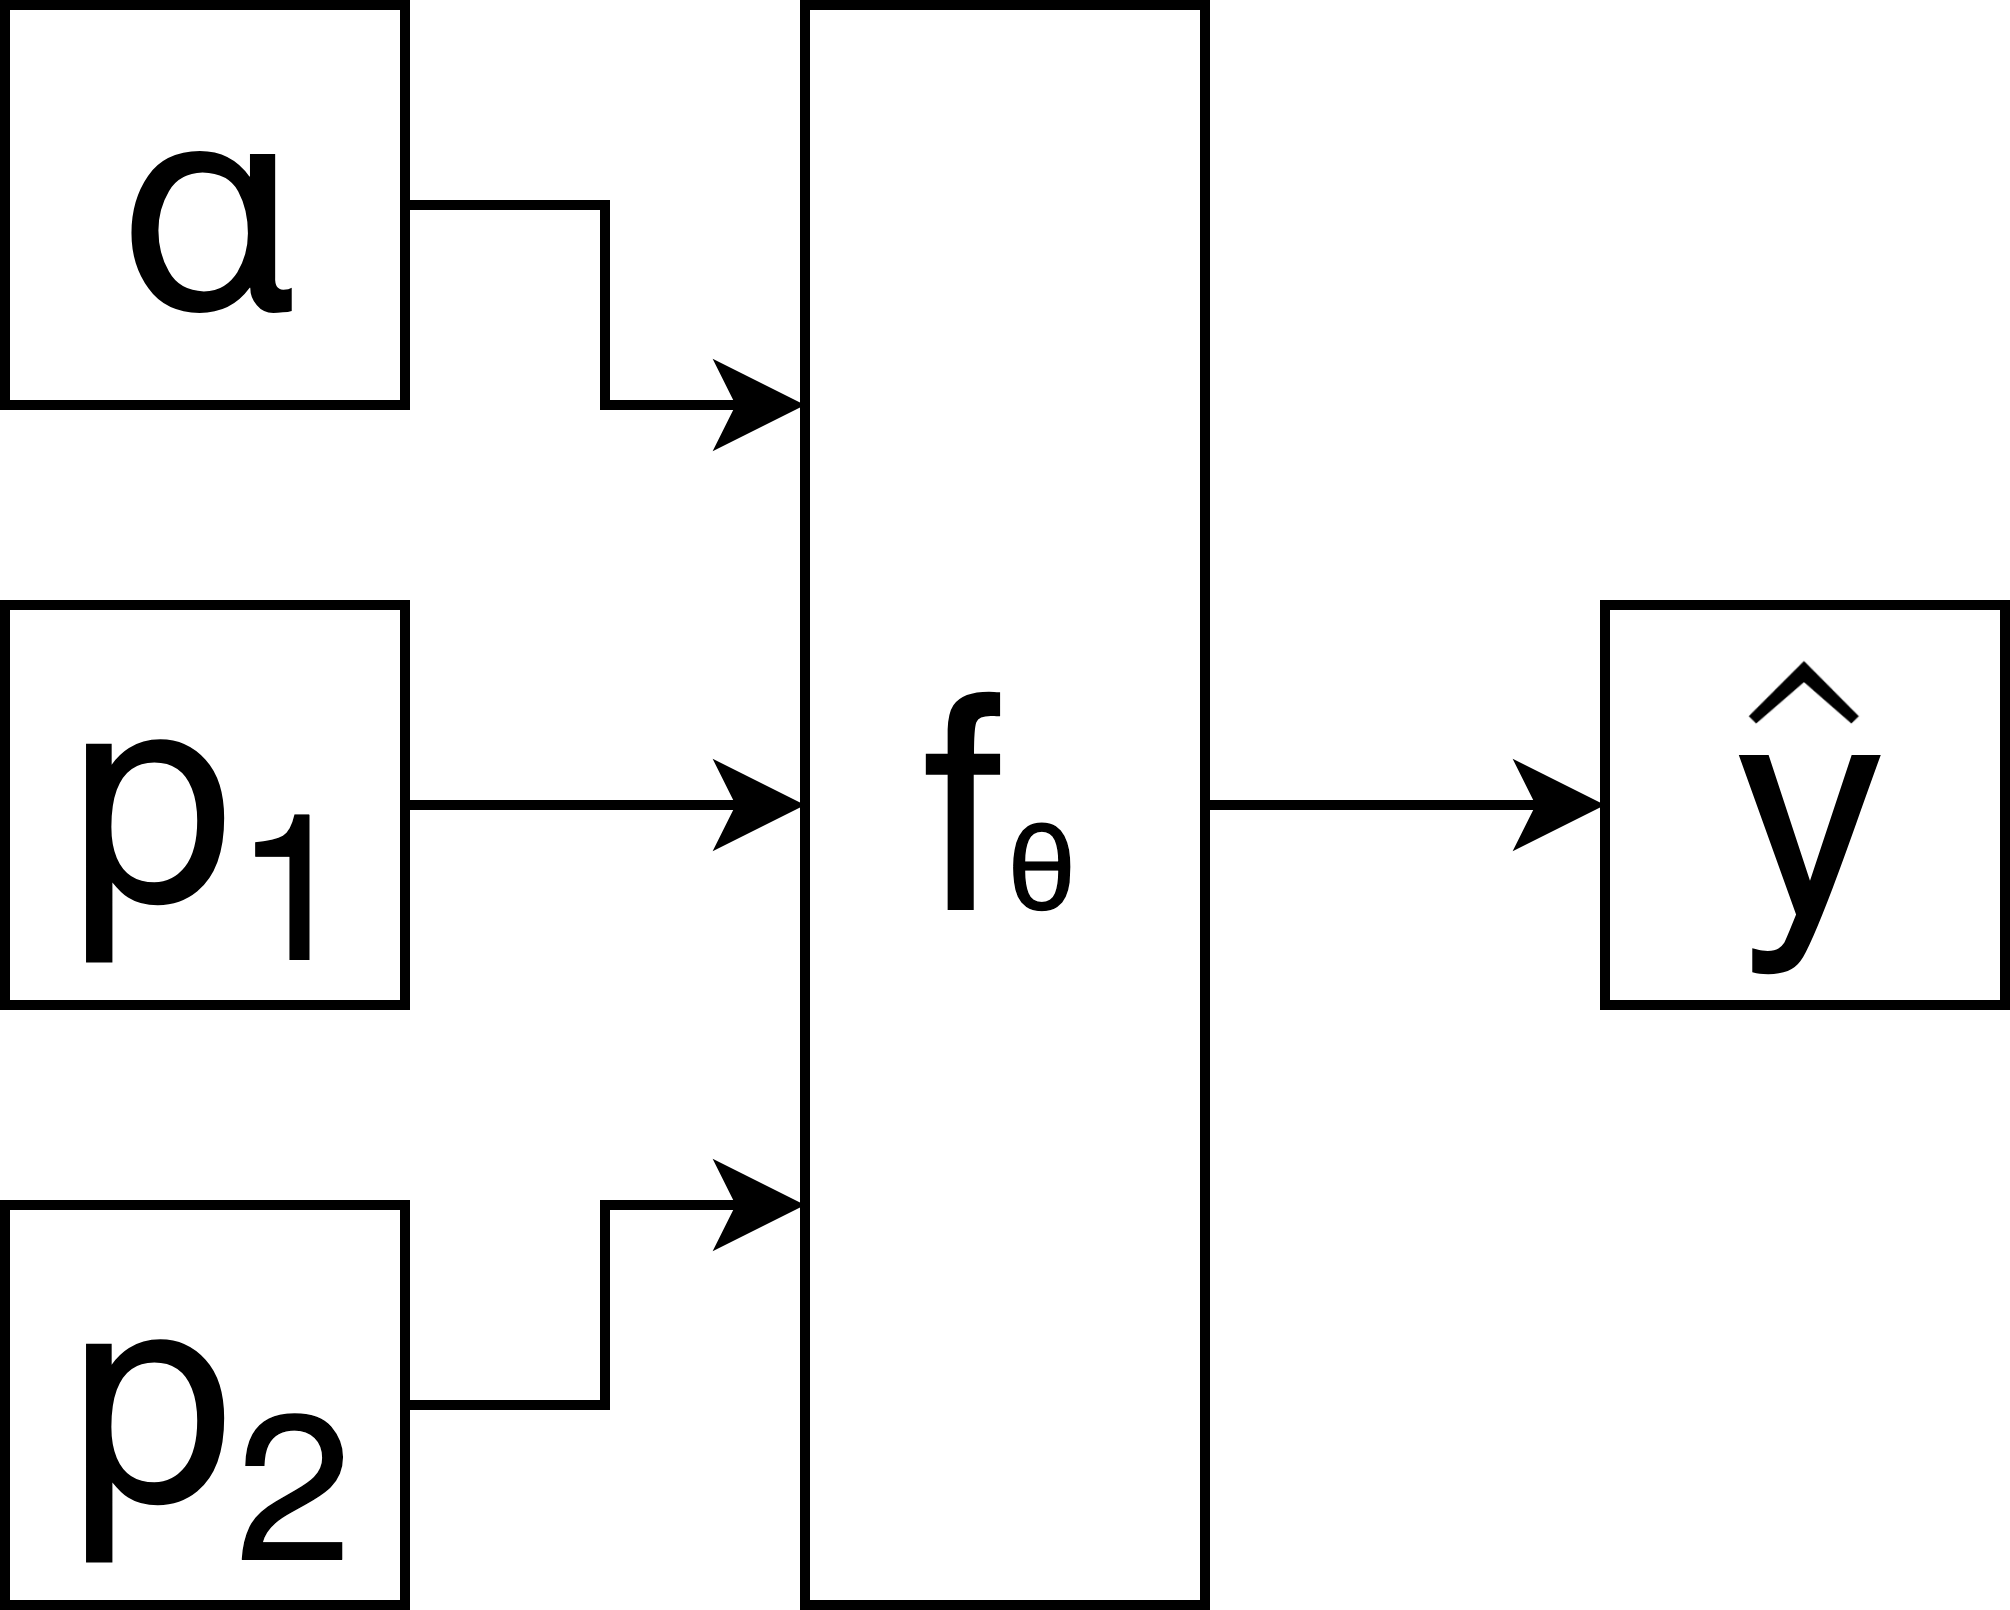
\includegraphics[height=2.5cm]{arch_model1}} & 
		\addvbuffer[2pt 0pt]{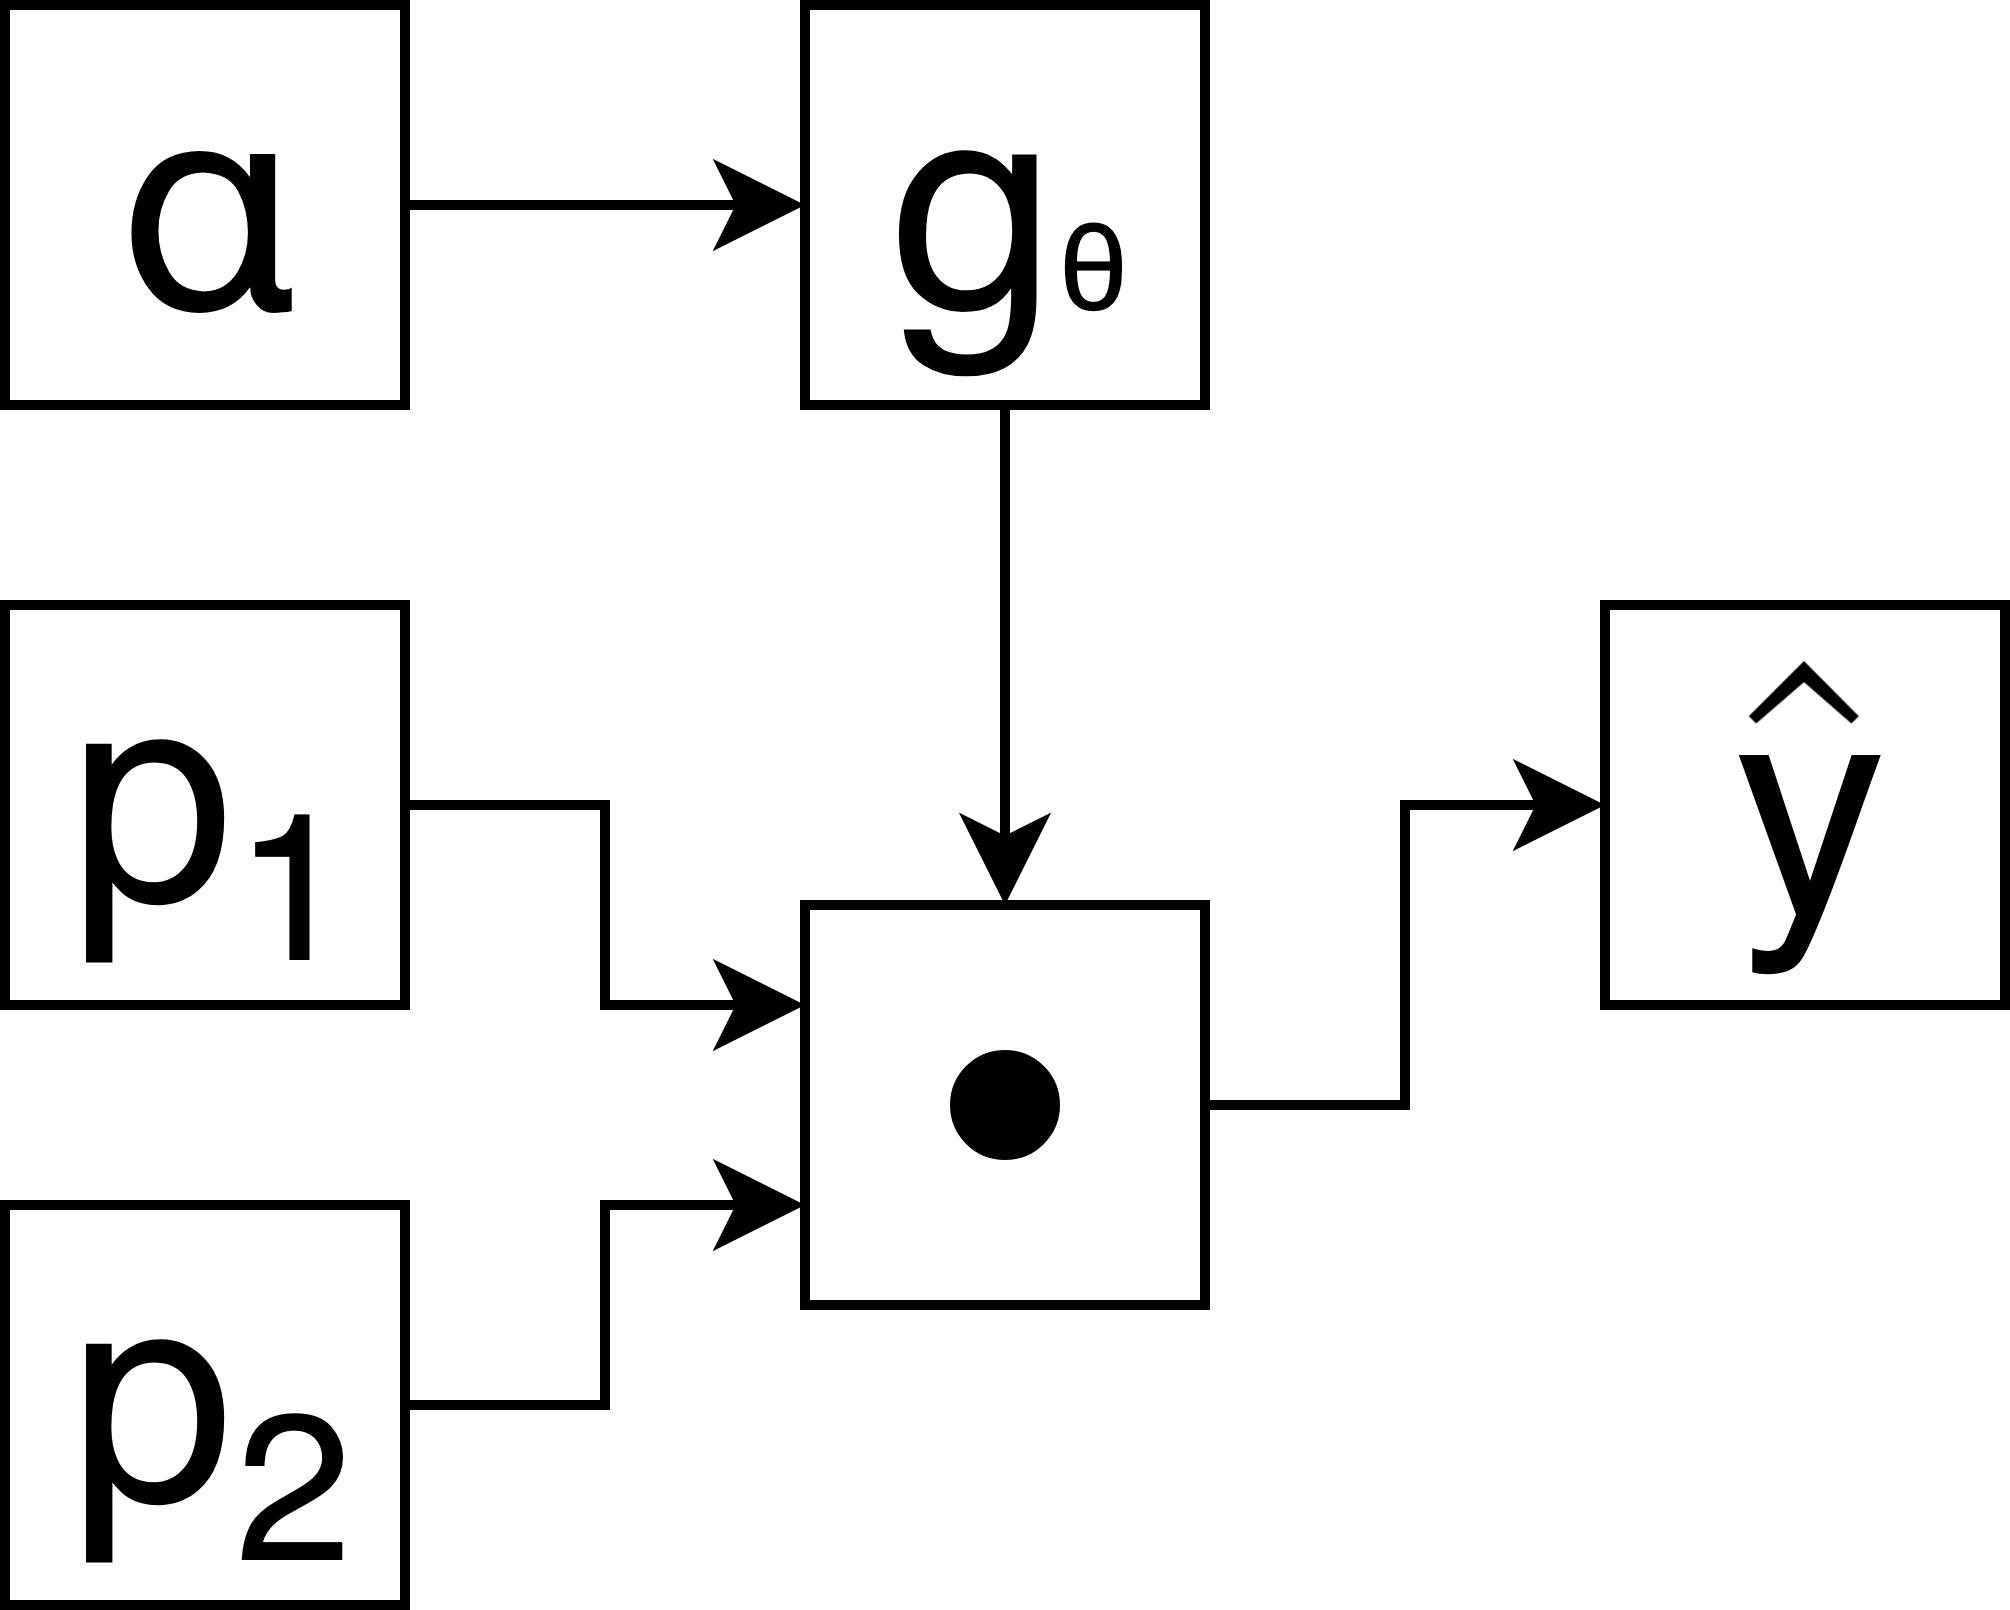
\includegraphics[height=2.5cm]{arch_model2}}  & 
		\addvbuffer[2pt 0pt]{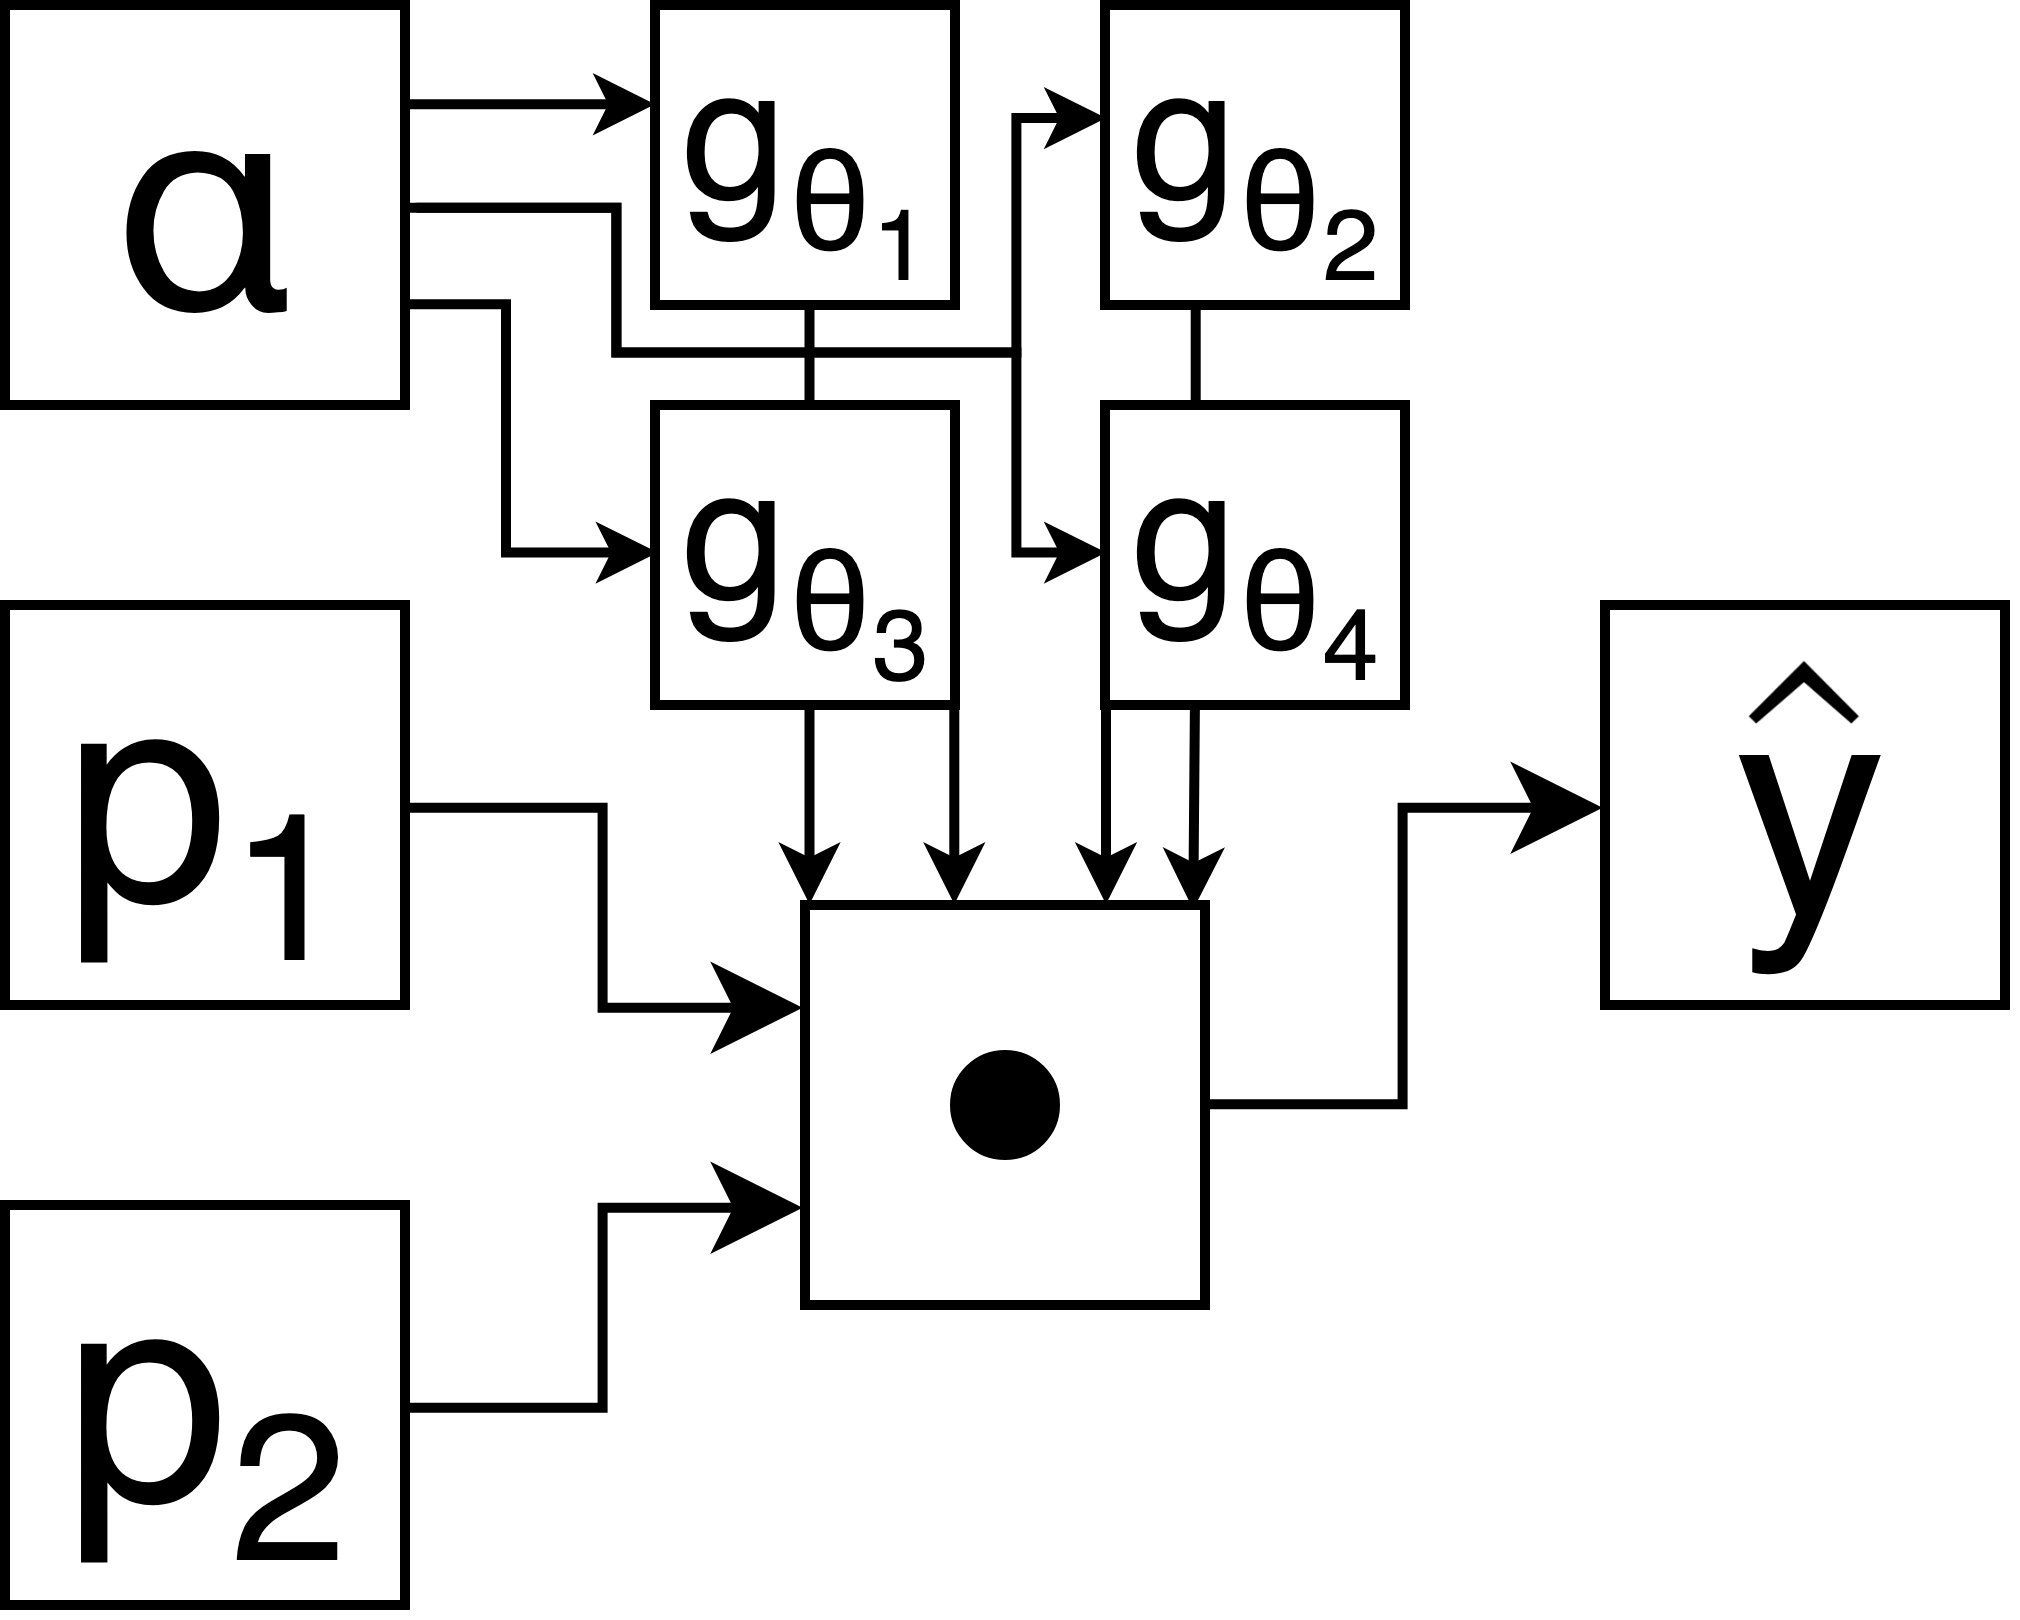
\includegraphics[height=2.5cm]{arch_model3}}  \\ 
		\hline
		\addvbuffer[3pt 0pt]{\shortstack{Network \\ function}} & 
		\addvbuffer[0pt 5pt]{$f_\theta: \mathbb{R}^3 \to \mathbb{R}^2$} & 
		\addvbuffer[0pt 5pt]{$g_\theta: \mathbb{R} \to \mathbb{R}^{2\times2}$} & 
		\addvbuffer[0pt 5pt]{$g_{\theta_i}: \mathbb{R} \to \mathbb{R}, i \in \{0, 1, 2, 3\}$} \\ 
		\hline
		Layer sizes & 
		$3 \to 16 \to 16 \to 16 \to 2$ &
		$1 \to 100 \to 4$ &
		$[1 \to 50 \to 1] \times 4$ \\
		\hline
		Activation & 
		Tanh &
		Sigmoid &
		Sigmoid \\
		\hline
		Parameters & 
		642 &
		604 &
		604 \\
		\hline
	\end{tabular}
\end{table}

\paragraph{Model 1:}The first model is a neural network directly approximating $f_\theta$. Thus, it takes a point of dimension $d$ and angles of dimension $d-1$ as input and predicts a target point of dimension $d$. The network has three hidden layers with 16 nodes each. In each of the hidden layers, the activation function $\tanh$ is applied.\\

For \textbf{Model 2} and \textbf{Model 3}, we make use of the knowledge that a rotation is the result of multiplying a rotation matrix, which only depends on the angles $\alpha$, with the given point $\vec{x}$. Consequently, the networks of the next models represent the function $g_\theta: [-\pi, \pi]^{d-1} \to \mathbb{R}^{d \times d}$, which in turn is used to create the final predictions in the following way:
\begin{equation}
\label{eq:rot_pred}
\hat{y} = g_\theta(\alpha) \, \vec{x},
\end{equation}
where $\alpha \in [-\pi, \pi]^{d-1}$ is the rotation angle and $\vec{x} \in \mathbb{R}^d$ the point to be rotated.

\paragraph{Model 2:} Based on this approach, the second model predicts the rotation matrix. In particular, it maps $d-1$ input angles to a matrix of size $d \times d$. This is done using one hidden layer of size 100 with the Sigmoid activation function. 

\paragraph{Model 3:} Similar to the previous model, we also try to solve the problem using an independent neural network for each of the $d \times d$ matrix entries. Each of these networks maps the rotation angles of size $d-1$ to a single real number, which is interpreted as a single matrix entry. For each of these networks, we use one hidden layer of size 50 with the Sigmoid activation function.\\

\subsection{Hyperparameters}
All layers of the neural networks include bias and we do not apply dropout. In order to achieve undistorted comparisons of the models, they were designed to have between 600 and 650 parameters each for the two-dimensional problem. For all experiments, we decide to use the Adaptive Moment Estimator "Adam" as our optimiser, since it empirically appeared to perform well in practice and is favourable to other known adaptive learning-method algorithms \cite{DBLP:journals/corr/Ruder16}. Furthermore, we use a learning rate of $5\times 10^{-5}$ and train each model using $50\,000$ iterations. Both of these parameters are empirically estimated, a comparison of using different learning rates on Model 3 is displayed in Figure \ref{fig:comp_lr_m3} in the appendix. For all experiments, we use a batch size of 512 and shuffle the training set at the start of each epoch.

\subsection{Metrics}
In the following, we introduce different loss functions to measure the desired properties of the predictions. The choice of these loss functions is critical, since they determine the objective function which is minimised in the training process. In particular, the loss functions need to measure the predictions' accuracy and physical feasibility.
\subsubsection{Accuracy}
As explained previously, the MSE Loss defined in equation \eqref{eq:mse} is a well fitting function to measure the accuracy of the predictions, since it is the sum of the square distances between the predictions and the corresponding target points. Hence, training on the MSE Loss aims to reduce this distance.
\subsubsection{Phyiscal feasibility}
In order to train our models to learn the physical constraints, we introduce loss functions specifically designed to measure how realistic the model predictions are. In general, our physical loss functions map the predicted points and, if applicable, the predicted rotation matrix to a real number, which is interpreted as the violation of the physical constraints. Thus, the physical loss functions are of the form
\[L_{PHY}: \mathbb{R}^d \times \mathbb{R}^{d \times d} \to \mathbb{R}. \]
\paragraph{Determinant constraint} 
In order to measure how well the predicted rotation matrices align with the constraint of the determinant being equal to one \eqref{eq:constraint_det}, we use the following function as our physical loss:
\[L_{DET}(\hat{y}, \hat{R}) = \frac{1}{N_{train}}\sum_{n = 1}^{N_{train}}(\det(\hat{R}_n) - 1)^2,\]
where $\hat{R}$ are the predicted rotation matrices computed by applying $g_\theta$ to each element of $X_{train}$. This can also be described as the MSE Loss between the vector of the predicted matrices' determinants and a vector of the same size filled with ones.
\paragraph{Norm constraint} 
In order to incorporate the constraint that the norm of any prediction needs to be one \eqref{eq:constraint_norm}, the following physical loss function is applied:
\[L_{NORM}(\hat{y}, \hat{R}) = \frac{1}{N_{train}}\sum_{n = 1}^{N_{train}}(||\hat{y}_n||_2 - 1)^2, \]
where $\hat{y}$ denotes the points predicted by the model. Similar to the Determinant loss, the Norm loss can be interpreted as the MSE Loss between the vector of the norms of the predictions and a vector of ones of the same size.

\subsection{Solving methods}
In this section, we will introduce the methods we apply to incorporate the physical loss functions into the models. As a baseline for comparisons, we train each model using solely the MSE Loss on the training data.

\subsubsection{Penalty Method}
The first and simplest version of the Penalty Method we apply is setting a fixed weight $\lambda > 0$ and solving a single minimisation problem, that is,

\[\underset{\theta}\argmin \,\, (\mathcal{L}_{MSE}(\hat{y}_\theta, y_{train}) + \lambda \cdot L_{PHY}(\hat{y}_\theta, g_\theta(X_{train}))).\]

In addition, we also solve a series of minimisation problems of the type above with exponentially increasing $\lambda$, but using the solution of the last iteration as a warm start for the next one. In particular, we introduce a multiplier $\mu > 1$ such that the weight of the physical loss in the i-th iteration is given by $\lambda_i = \mu^i \, \lambda_0$. Each minimisation is stopped as soon as the norm of the gradient is below a certain threshold.

\subsubsection{Augmented Lagrangian Method}
\label{exp:alm}
As we do for the Penalty Method, we also apply two different versions of the Augmented Lagrangian Method. Both versions minimise a fixed number of problems and update the weights of the linear constraint terms according to rule \eqref{eq:alm_update}. However, the first one only computes a fixed number of epochs with a constant weight $\lambda$ for the physical loss for each minimisation problem.\\
\indent The second version was suggested by Bertsekas in \cite{Yurkiewicz1985ConstrainedOA}. In addition to increasing the weight of the squared constraint term, he proposes to stop the minimisation of the k-th problem as soon as the norm of the gradient is smaller than a threshold $\tau_k$ computed according to the following equation:
\[\tau_k = \min(\epsilon_k, \gamma_k ||c(x_k)||_2), \]
where $\{\epsilon_k\}$ and $\{\gamma_k \}$ are two sequences decreasing to 0 and $c(x_k)$ is the value of the constraint violation at the current solution. In our experiment, $c(x_k)$ is the difference of the norms / determinants of the predicted points / rotation matrices and one. Intuitively, this approach spends more ressources on minimising a problem if the predictions of the current solution already align well with the physical constraints and otherwise focuses on learning the constraints first.

\subsubsection{Physical Projection}
\label{sec:phys_proj}
As a third approach, we apply the Physical Projection. In particular, each prediction in the training process is projected to the closest feasible prediction. When applying it to the norm loss, we divide the predicted point $\hat{y}$ by its norm and thus get a prediction $\hat{y}'$ located on the unit circle or unit sphere. Formally, predictions are calculated the following way:
\begin{equation}
\hat{y}' = \frac{\hat{y}}{||\hat{y}||_2}.
\end{equation}

For the determinant, we only divide the matrix by the $d$-th root of the determinant if the latter is positive, otherwise we do not change the matrix. Therefore any predicted rotation matrix with a positive determinant is projected to a new matrix with a determinant of one. Formally, we update each predicted matrix $\hat{R}_n$ according to the following rule:
\begin{equation}
\hat{R}_n' = \begin{cases} \frac{\hat{R}_n}{\sqrt[d]{\det(\hat{R}_n)}}, \qquad \text{if} \det(\hat{R}_n) > 0 \\ \hat{R}_n, \qquad \qquad \,\,\,\,\text{else} \end{cases}, \qquad n = 1, ..., N_{train}.
\label{eq:norm_det}
\end{equation}

Since matrices with negative determinants are far away from the true rotation matrix, they should not occur often or if so, be corrected by solely training on the MSE-Loss for the prediction and the target point. 

\subsection{Statistical measurements}
Each experiment will be tested on 20 different seeds used to generate the training data, with a few exceptions due to time limitations. If not otherwise specified, we compare the performance of the models according to the mean of the MSEs of the individual runs. We prefer the mean over the median, because we are also interested in the performance of outliers that lead to poor results. The test set on which each model's performance is calculated consists of 4096 data points sampled in the same manner as the training dataset.\\








\clearpage

